\documentclass[conference]{IEEEtran}
\usepackage{cite}
\usepackage{amsmath,amssymb,amsfonts}
\usepackage{graphicx}
\usepackage{booktabs}
\usepackage{textcomp}
\usepackage{xcolor}
\usepackage{hyperref}
\hypersetup{colorlinks=true,linkcolor=blue,citecolor=blue,urlcolor=blue}

\begin{document}

\title{When Do Hierarchical Constraints Help? A Systematic Study of R-Matrix Consistency and Reconciliation in Hierarchical Multi-Label Classification}

\author{\IEEEauthorblockN{Bruno Sette\IEEEauthorrefmark{1} and [Orientador]\IEEEauthorrefmark{1}}
\IEEEauthorblockA{\IEEEauthorrefmark{1}Federal University of S\~ao Carlos (UFSCar), S\~ao Carlos, SP, Brazil\\
Email: brunosilvasette@gmail.com, [orientador@ufscar.br]}}

\maketitle

\begin{abstract}
Hierarchical multi-label classification (HMC) requires predictions to be
consistent with a class hierarchy: an ancestor must not score lower than its
descendants. The R-matrix constraint enforces this property, but prior work
evaluates it together with a specific architecture and training recipe, so it
is unclear whether the benefit comes from the training-time consistency loss,
from inference-time reconciliation, or from the architecture. We isolate these
factors in a controlled study of three objectives (BCE, hinge, and MCLoss)
with and without reconciliation on 27 datasets---text, FunCat, Gene Ontology,
and cross-domain ARFF---under a validation-only protocol. We also introduce a
sparse $O(C{+}E)$ formulation of the R-matrix that avoids the dense
$C\times C$ tensor. The main finding is that \emph{reconciliation at inference
time} drives the gains, not the consistency loss during training: BCE with
reconciliation is competitive with MCLoss, and MCLoss raw scores can collapse
before reconciliation. On FunCat and Gene Ontology the approach is on par with
C-HMCNN (0.259/0.261 vs.\ 0.264 and 0.416/0.418 vs.\ 0.420 AUPRC on the
datasets with published baselines), and on cross-domain ARFF it improves over
C-HMCNN on three of four datasets (0.857 vs.\ 0.849). On WOS it reaches 0.8704
$\pm$ 0.0033 micro-F1, 0.0012 below HPT. The sparse formulation scales to DAGs
with 4{,}134 classes, and a reproduction study shows that the reported Surj
results cannot be verified from the published description. Code and artifacts
are available at \url{https://github.com/Sette/hmc-torch}.
\end{abstract}

\begin{IEEEkeywords}
hierarchical multi-label classification, R-matrix, hierarchical consistency,
reconciliation, reproducibility
\end{IEEEkeywords}

\section{Introduction}
\label{sec:intro}

Hierarchical multi-label classification (HMC) assigns each instance to one or
more nodes of a predefined class hierarchy, a tree or a directed acyclic graph
(DAG). It appears in scientific text categorization (ArXiv, WOS), protein
function prediction (Gene Ontology), and cross-domain taxonomy annotation.
Beyond flat multi-label accuracy, HMC requires \emph{hierarchical consistency}:
if a model predicts a descendant, it should predict its ancestors as well.

The R-matrix constraint~\cite{chmcnn} enforces this property by making an
ancestor's score at least the maximum over its descendants. It has been
implemented in two places: a differentiable \emph{training-time consistency
loss} (a hinge or the MCLoss of C-HMCNN) and an \emph{inference-time
reconciliation} that propagates scores bottom-up. Published HMC systems
usually report the combination of both, entangled with a particular
architecture and training recipe. As a result, it is unclear whether the
constraint helps because of the loss, because of the post-hoc reconciliation,
or because the model that carries the constraint is simply better tuned. A
second obstacle is scale: materializing the dense $C\times C$ R-matrix is
prohibitive for ontologies with thousands of classes.

This paper isolates the two mechanisms. We ask: (Q1) does the training-time
consistency loss improve over plain BCE? (Q2) does inference-time
reconciliation drive the gain? (Q3) can the constraint scale to large DAGs?
We answer with a controlled study of three objectives (BCE, hinge, and MCLoss)
$\times$ \{raw, reconciled\} on 27 datasets, using a validation-only protocol:
early stopping and the decision threshold are chosen on validation, and the
test split is used once.

Our contributions are:
\begin{itemize}
  \item A \textbf{sparse $O(C{+}E)$ formulation} of the R-matrix that preserves
  the constraint on large DAGs without materializing the dense matrix.
  \item A \textbf{controlled study} of three objectives with and without
  reconciliation on 27 datasets spanning text, genomic tabular data, Gene
  Ontology, and cross-domain ARFF.
  \item The \textbf{central finding} that reconciliation at inference time,
  not the training-time loss, is what moves the scores; BCE with reconciliation
  is competitive with MCLoss, whose raw scores can collapse.
  \item \textbf{Negative and reproducibility results}: the reported Surj
  numbers cannot be verified from the published description, and autoencoder
  branches add no consistent gain.
  \item An open-source implementation that makes the study reproducible.
\end{itemize}
We credit the R-matrix idea to Giunchiglia and Lukasiewicz~\cite{chmcnn}; our
contribution is the sparse formulation, the systematic isolation, and the
empirical conclusions.

\section{Related Work}
\label{sec:related}

Early HMC methods train local classifiers per level or per node~\cite{silla2011hmc,cerri2014hmc}.
Global methods predict all classes jointly: HMCN~\cite{weihs2018hmc} couples
levels with a recurrent architecture, and C-HMCNN~\cite{chmcnn} introduces the
R-matrix constraint. In hierarchical text classification, HiAGM~\cite{zhou2020hiagm}
uses a GCN over the label hierarchy, HTCInfoMax~\cite{htcinfomax} adds mutual
information maximization, HGCLR~\cite{hgclr} injects hierarchy into the text
encoder, HPT~\cite{hpt} uses hierarchy-aware prompt tuning, and
HiMatch~\cite{himatch} matches label semantics. Surj~\cite{www2022ontology}
learns label embeddings with a graph autoencoder and reports the highest
FunCat/GO numbers, but its code was never released.

Two gaps motivate this paper. First, the constraint is usually evaluated
jointly with the architecture and recipe, so the attribution between the
training loss and inference reconciliation is not isolated. Second, dense
R-matrix implementations are $O(C^2)$ in memory, which limits their use on
large ontologies such as Gene Ontology (thousands of classes). Our study
addresses both with a sparse formulation and a factorial evaluation.

\section{Method}
\label{sec:method}

\subsection{The R-matrix}
Let $A$ be the hierarchy adjacency matrix with $A_{ij}=1$ if $i$ is a direct
child of $j$ (edges point child $\rightarrow$ parent). The R-matrix is the
transitive closure
\begin{equation}
R_{ij} = \begin{cases}
1 & \text{if } i=j \text{ or } \exists \text{ path } j \rightarrow \ldots \rightarrow i,\\
0 & \text{otherwise,}
\end{cases}
\label{eq:rmatrix}
\end{equation}
so $R_{ij}=1$ iff $i$ is an ancestor of $j$. Hierarchical consistency requires
$p_i \ge p_j$ whenever $R_{ij}=1$.

\subsection{Training objectives}
We compare three objectives:
\begin{itemize}
  \item \textbf{BCE}: plain binary cross-entropy on the labels.
  \item \textbf{Hinge}: BCE plus a penalty over ancestor--descendant pairs,
  \begin{equation}
  \mathcal{L}_{\text{hier}} = \frac{1}{B|R|}\sum_{b=1}^{B}\sum_{i,j:R_{ij}=1}
  \max(0,\,p_{b,j}-p_{b,i}+\gamma),
  \label{eq:hinge}
  \end{equation}
  with margin $\gamma=0$.
  \item \textbf{MCLoss}: C-HMCNN's loss~\cite{chmcnn}, i.e.\ BCE computed on
  the max-constrained outputs $\max(p_i,\max_{j:\text{child}(i,j)}p_j)$.
\end{itemize}

\subsection{Inference-time reconciliation}
At prediction time we enforce the hard constraint bottom-up:
\begin{equation}
p_i^{\text{rec}} = \max\Big(p_i,\ \max_{j\in\text{children}(i)} p_j^{\text{rec}}\Big),
\label{eq:reconcile}
\end{equation}
processing levels from deepest to shallowest. Leaves keep their scores; only
internal nodes can change. Reconciliation is applied identically to every
objective, so ``raw'' and ``reconciled'' isolate its effect.

\subsection{Sparse R-matrix}
The dense R-matrix stores $C^2$ entries. For Gene Ontology, $C\approx 4{,}000$
and the $B\times C\times C$ tensor exceeds GPU memory at batch 64. We store
only the parent--child edges and a breadth-first ordering of the nodes, and
propagate scores bottom-up along the graph. The memory cost is $O(C{+}E)$; for
\texttt{cellcycle\_GO} ($C=4{,}126$, $E=5{,}827$) this reduces the constraint
storage from 65~MB to about 46~KB ($>1{,}400\times$). The sparse
\texttt{BlockDiagonalR} reproduces the dense max propagation exactly, and it is
differentiable, so the same operator serves both the loss and reconciliation.

\section{Experimental Setup}
\label{sec:setup}

\begin{table}[t]
\caption{Datasets evaluated in this paper (27).}
\label{tab:datasets}
\centering
\footnotesize
\begin{tabular}{lccc}
\toprule
Family & \# & Classes & Hierarchy \\
\midrule
Text & 4 & 62--4{,}520 & tree/DAG \\
FunCat & 10 & 456--500 & tree \\
Gene Ontology & 9 & 3{,}128--4{,}134 & DAG \\
Cross-domain ARFF & 4 & 47--399 & tree \\
\bottomrule
\end{tabular}
\end{table}

\textbf{Datasets.} We use 27 datasets in four families: (i) text---ArXiv,
WOS, AAPD, and EUR-Lex 57K (4,271 dataset concepts; 4,519 evaluated
hierarchy nodes; text = title + header + recitals + main body, truncated to 256
tokens); (ii) 10 FunCat genomic datasets (tree hierarchy);
(iii) 9 Gene Ontology datasets (DAG with up to 4{,}134 classes); and (iv) four
cross-domain ARFF datasets (Enron email, Diatoms microscopy, and ImCLEF07a/d
medical imaging). RCV1-V2 is supported by the implementation but pending the
NIST license. Text uses SPECTER2-base (768-d, CLS pooling, 256-token
limit), frozen or
fine-tuned; ARFF features are pre-extracted.

\textbf{Protocol.} We train on the training split; early stopping and the
decision threshold are chosen on validation (sweep 0.05--0.95); the test split
is used once. On ARFF datasets the model is refit on training + validation for
the selected number of epochs, following HMCN and C-HMCNN; on text it is not
refit, following HPT. All results are means over seeds 0, 42, and 123. We
report micro-F1 (text) and micro-AUPRC (FunCat/GO), plus AUPRC for
cross-domain. Baselines come from their papers; Surj's reported numbers are
listed but excluded from rankings because they cannot be verified.

\textbf{Training details.} FunCat/GO: three-layer MLP, hidden size from the
registry, dropout 0.7, batch 4, AdamW (LR $10^{-4}$, weight decay $10^{-5}$),
early stopping on validation AUPRC (patience 20, at most 200 epochs), then
refit on training + validation for the selected number of epochs. Text:
SPECTER2-base, CLS pooling, 256-token limit; frozen features with an MLP, or end-to-end
fine-tuning on WOS (transformer LR $2\times10^{-5}$, classifier LR $10^{-4}$,
batch 8, 10 epochs, epoch and threshold on validation). Cross-domain ARFF: the
FunCat recipe with dropout 0.3 and batch 32. All runs use an RTX 3060.

\section{Results}
\label{sec:results}

\subsection{FunCat and Gene Ontology}
Table~\ref{tab:main} summarizes the 8 FunCat and 8 GO datasets that have
published baselines (church/pheno\_FUN and pheno\_GO have none). On FunCat our
best configuration (MCLoss + graph autoencoder) averages 0.262 against 0.264
for C-HMCNN; on GO, MCLoss averages 0.418 against 0.420 for C-HMCNN and 0.422
for HMCN-F. The three objectives are within 0.002 of each other on both
families: the training-time loss does not separate them. The same constraint
through the sparse R formulation is enough to reach the published baselines.
A graph-autoencoder branch adds +0.002 AUPRC on FunCat (0.262 vs.\ 0.261) but
was not run on GO, where the screening gain was below 0.003. F1 falls with
depth on every family; the deepest, sparsest levels are the hardest, and that
is where reconciliation changes the most predictions.

\begin{table}[t]
\caption{AUPRC on the 8 FunCat and 8 GO datasets with published baselines
(mean of 3 seeds, reconciled outputs).}
\label{tab:main}
\centering
\footnotesize
\begin{tabular}{lcc}
\toprule
Method & FunCat & GO \\
\midrule
C-HMCNN (NeurIPS'20)~\cite{chmcnn} & \textbf{0.264} & 0.420 \\
HMCN-F (ICML'18)~\cite{weihs2018hmc} & 0.261 & \textbf{0.422} \\
Ours BCE + rec. & 0.259 & 0.416 \\
Ours hinge + rec. & 0.259 & 0.417 \\
Ours MCLoss + rec. & 0.261 & 0.418 \\
Ours MCLoss + GAE + rec. & 0.262 & -- \\
Ours GBDT + rec. & 0.226 & -- \\
\bottomrule
\end{tabular}
\end{table}

\subsection{Where the gain comes from}
Figure~\ref{fig:decomp} decomposes the result into BCE only, training-time
consistency loss (MCLoss without reconciliation), inference reconciliation
only (BCE + rec.), and both. The pattern is consistent across the three
panels: training with the loss alone is never better than BCE, while
reconciliation moves the scores. On ArXiv, MCLoss raw (0.715) is below BCE raw
(0.722), but both reach 0.723--0.724 after reconciliation. On
\texttt{cellcycle\_GO}, MCLoss raw (0.409) is far below BCE raw (0.433), and
reconciliation brings it to 0.437, slightly above BCE + rec.\ (0.433). The
constraint is therefore useful mainly as an inference-time prior; its
training-time loss is not a reliable source of gain.

\begin{figure*}[t]
\centering
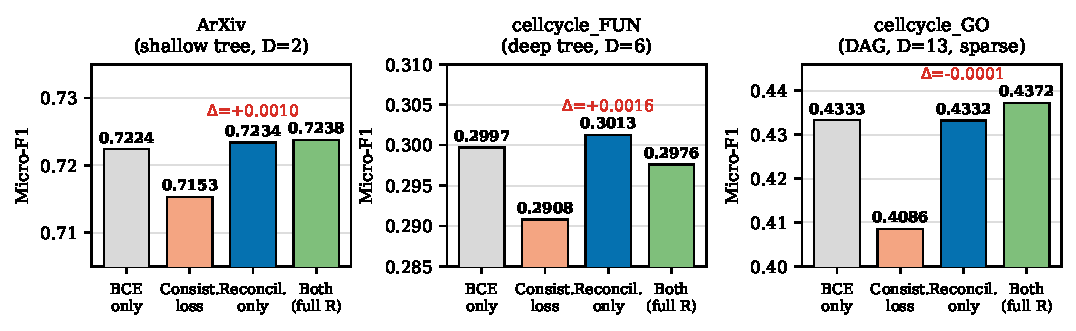
\includegraphics[width=\textwidth]{figures/fig_ablation.pdf}
\caption{R-matrix decomposition on ArXiv, \texttt{cellcycle\_FUN}, and
\texttt{cellcycle\_GO}: plain BCE, training-time consistency loss (MCLoss
without reconciliation), inference-time reconciliation only (BCE + rec.),
and both. Training with the loss alone is not better than BCE; reconciliation
is what moves the scores. Mean of 3 seeds.}
\label{fig:decomp}
\end{figure*}

\subsection{Scaling to Gene Ontology}
The sparse formulation runs on all 9 GO datasets, up to 4{,}134 classes, with
the same accuracy as the dense max propagation. For \texttt{cellcycle\_GO}
($C=4{,}126$, $E=5{,}827$) the dense constraint needs 65~MB per batch and does
not fit at batch 64; the sparse version uses about 46~KB and trains at that
batch size. This is what makes the systematic comparison on GO possible.

\begin{figure}[t]
\centering
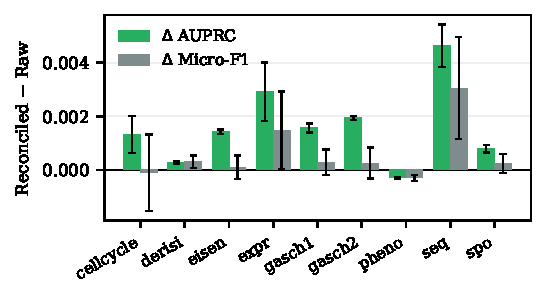
\includegraphics[width=\columnwidth]{figures/fig3_go_sparse.pdf}
\caption{AUPRC on the 9 Gene Ontology datasets with the sparse R-matrix,
raw versus reconciled. Reconciliation improves 8 of 9 datasets; the sparse
operator is exact and trains at batch 64.}
\label{fig:go}
\end{figure}

\subsection{Text and cross-domain}
Table~\ref{tab:text} reports the remaining families. On WOS, fine-tuned
SPECTER2 with the constraint reaches 0.8704 $\pm$ 0.0033 micro-F1, 0.0012 below
HPT (0.8716) and 0.0007 below HGCLR (0.8711); frozen features give 0.7462.
HiAGM and HTCInfoMax are HPT's BERT re-executions on the same split; HGCLR
and HPT are as reported in their papers. On
ArXiv, AAPD, and EUR-Lex the results are competitive under their respective
splits, but the comparisons are not like-for-like (different splits and
baselines), so we do not claim a margin. On the cross-domain ARFF datasets our
BCE + rec.\ model averages 0.857 against 0.849 for C-HMCNN and 0.781 for
HMCN-F, with the largest gain on Diatoms (+0.027). MCLoss is worse than BCE on
three of four cross-domain datasets in the raw scores, and reconciliation
recovers most of the gap---the same pattern as Figure~\ref{fig:decomp}.

\begin{table}[t]
\caption{Micro-F1 on WOS under the HPT protocol (30{,}070/7{,}518/9{,}397).}
\label{tab:wos}
\centering
\footnotesize
\begin{tabular}{lc}
\toprule
Method & Micro-F1 \\
\midrule
HiAGM (ACL'20)~\cite{zhou2020hiagm} & 0.8604 \\
HTCInfoMax (NAACL'21)~\cite{htcinfomax} & 0.8630 \\
HGCLR (ACL'22)~\cite{hgclr} & 0.8711 \\
HPT (EMNLP'22)~\cite{hpt} & \textbf{0.8716} \\
Ours (fine-tuned + R) & 0.8704 $\pm$ 0.0033 \\
\bottomrule
\end{tabular}
\end{table}

\begin{table}[t]
\caption{Text (micro-F1) and cross-domain (AUPRC) results, mean of 3 seeds.
Text comparisons are not like-for-like except WOS.}
\label{tab:text}
\centering
\footnotesize
\begin{tabular}{lc}
\toprule
Setting & Value \\
\midrule
WOS frozen & 0.7462 \\
ArXiv (own split) & 0.7234 \\
AAPD (own split) & 0.8232 \\
EUR-Lex 57K (standard split) & 0.7888 \\
\midrule
Cross-domain avg & \textbf{0.857} \\
\quad C-HMCNN / HMCN-F & 0.849 / 0.781 \\
\quad hinge + rec. & 0.855 \\
\quad MCLoss + rec. & 0.853 \\
\bottomrule
\end{tabular}
\end{table}

\subsection{Reproducibility}
Surj~\cite{www2022ontology} is the only published model above the
constraint-based methods on FunCat and GO, but its code was never released. We
reimplemented it on C-HMCNN's pipeline and chose the unreported hyperparameters
on validation. It averages 0.232 on FunCat (vs.\ 0.312 reported) and 0.352 on
GO (vs.\ 0.468), staying below C-HMCNN. Without the authors' code, those
numbers cannot be verified; we list them as reported and exclude them from
every ranking.

\section{Discussion and Limitations}
\label{sec:discussion}

\textbf{When does the constraint help?} The clearest gains appear when the
hierarchy is clean and the domain shifts: the cross-domain ARFF benchmarks gain
+0.008 on average over C-HMCNN, with Diatoms at +0.027. On FunCat and GO the
constraint reaches parity with the published baselines, and on text it is
competitive but not state of the art. The practical lesson is to use
reconciliation at inference time and not to expect the training-time loss to
provide the gain by itself.

\textbf{Practical guidance.} (i) Apply reconciliation at inference: it is
cheap and drives most of the gain. (ii) Do not expect the training-time loss to
beat BCE; use it only when the architecture already benefits. (iii) Above a few
thousand classes, use the sparse $O(C{+}E)$ formulation; the dense
$C\times C$ tensor becomes the bottleneck. (iv) Report raw and reconciled
scores separately---the decomposition is the informative result.

\textbf{Limitations.} The gains are small, and several are within seed noise.
The text comparisons use our own splits (ArXiv, AAPD), so they are not
like-for-like; EUR-Lex has a deep hierarchy (29% internal labels) but
reconciliation changes only 10.7% of the internal scores; RCV1-V2 is
pending license; most published baselines are taken from their papers,
while we reproduce C-HMCNN's pipeline within 0.003 AUPRC on FunCat as a
sanity check. These are natural next steps, together with a prompt-based
hierarchy encoder.

\textbf{Threats to validity.} The ArXiv and AAPD splits are ours, not canonical
releases, so their numbers are not directly comparable to published systems;
WOS is the only like-for-like text comparison. Most published baselines
are taken from their papers; C-HMCNN's pipeline is reproduced within 0.003
AUPRC, and Surj's numbers are unverifiable. The gains are small and, in
some datasets, within seed variance;
we mitigate this by reporting means over three seeds and the raw/reconciled
decomposition. EUR-Lex has a deep hierarchy (29% internal labels), but
reconciliation changes only 10.7% of the internal scores there.

\section{Conclusion}
\label{sec:conclusion}

We isolated the R-matrix constraint in HMC. The sparse $O(C{+}E)$ formulation
scales the constraint to ontologies with thousands of classes, and the
controlled study shows that inference-time reconciliation, not the training
loss, is what improves the scores. BCE with reconciliation is competitive with
MCLoss, whose raw scores can collapse; on FunCat/GO the approach is on par with
C-HMCNN, and on cross-domain ARFF it improves on it. The code and artifacts
are released to make the study reproducible.

\section*{Availability}

The \texttt{hmc-torch} implementation, experiment configurations, per-seed
results, and the Surj reimplementation are available at
\url{https://github.com/Sette/hmc-torch} and
\url{https://pypi.org/project/hmc-torch/}.

\bibliographystyle{IEEEtran}
\bibliography{refs}

\end{document}
